\section{Multiple-Input-Multiple-Output Frequency-Modulated-Continuous-Wave Radar Signal Model}
\label{sec:mimo fmcw radar signal model}

The frequency-modulated-continuous-wave (FMCW) waveform is a popular choice for many radar applications due to its ability to simultaneously measure range and Doppler velocity. The FMCW waveform is a sinusoidal signal that increases in frequency linearly with time.

To start, a sinusoidal signal can be modeled as a complex exponential with phase $\phi(t)$ as a function of time $t$,

\begin{equation}
	m(t) = e^{j\phi(t)}.
\end{equation}

Recalling Euler's formula, the complex exponential can be expanded to sines and cosines as

\begin{equation}
	e^{j\phi(t)} = \cos(\phi(t)) + j\sin(\phi(t)).
\end{equation}

For a simple single tone sinusoid, $\phi(t) = 2\pi f_0 t$. Recalling the definition of instantaneous frequency as the derivative of the phase with respect to time and scaled by the reciprocal of $2\pi$, 

\begin{equation}
	\label{eq:instantaneous frequency}
	f(t) = \frac{1}{2\pi} \frac{\partial \phi(t)}{\partial t},
\end{equation}
the single tone sinusoid has a frequency of $f_0$ in Hz.

Thus, it follows that for a sinusoidal signal whose instantaneous frequency increases with time must have a quadratic phase, with respect to time.



\subsection{FMCW Signal Model}
\label{subsec:fmcw signal model}

Intuition of the FMCW signal model starts by considering a single transceiver consisting of a transmitter and receiver located $(x_T,y_T,Z_0)$ and $(x_R,y_R,Z_0)$, respectively with a single point target located at $(x_0,y_0,z_0)$. The transmitted signal is a linearly modulated chirp modeled by 

\begin{equation}
	\label{eq:transmitted signal}
	m(t) = e^{j2\pi(f_0t + 0.5Kt^2)}, \quad 0 \leq t \leq T,
\end{equation}
where $f_0$ is the starting frequency at time $t = 0$, $K$ is the chirp slope, and $T$ is the chirp duration. The instantaneous frequency and bandwidth of the FMCW chirp can be computed by

\begin{gather}
	\label{eq:fmcw frequency}
	f(t) = f_0 + Kt, \quad 0 \leq t \leq T, \\
	B = KT.
	\label{eq:fmcw bandwidth}
\end{gather}

Equation (\ref{eq:transmitted signal}) is transmitted by the transmit antenna (Tx), backscattered by the point reflector with reflectivity $\sigma$, and returns to the radar receiver as a scaled and time delayed version of the transmitted signal as

\begin{equation}
	\label{eq:received signal}
	\hat{m}(t) = \frac{\sigma}{R_T R_R} m(t-\tau_0) = \frac{\sigma}{R_T R_R} e^{j2\pi(f_0(t-\tau_0) + 0.5K(t-\tau_0)^2)},
\end{equation}
where $\tau_0$ is the round trip time delay $R_T$ is the distance from the transmitter to the point target, and $R_R$ is the distance from the receiver to the point target as

\begin{gather}
	R_T = \sqrt{(x_0 - x_T)^2 + (y_0 - y_T)^2 + (z_0 - Z_0)^2},\\
	R_R = \sqrt{(x_0 - x_T)^2 + (y_0 - y_T)^2 + (z_0 - Z_0)^2},\\
	\tau_0 = \frac{R_T + R_R}{c},
	\label{eq:tau_0}
\end{gather}
using $c$ as the speed of light.

The receives signal (\ref{eq:received signal}) is mixed with the transmitted signal (\ref{eq:transmitted signal}) yielding the IF signal or radar beat signal as

\begin{equation}
	\label{eq:beat signal full}
	s(t) = m(t)\hat{m}^*(t) = \frac{\sigma}{R_T R_R} e^{j2\pi(f_0\tau_0 + K\tau_0t - 0.5K\tau_0^2)}.
\end{equation}

The last phase term in the IF signal is known as the residual video phase (RVP) term and is known to be negligible. Under that assumption and using (\ref{eq:tau_0}) and (\ref{eq:fmcw frequency}), (\ref{eq:beat signal full}) can be rewritten as 

\begin{equation}
	s(t) = \frac{\sigma}{R_T R_R} e^{j2\pi(f_0 + Kt)(\frac{R_T + R_R}{c})} = \frac{\sigma}{R_T R_R} e^{j(\frac{2\pi f}{c})(R_T + R_R)}.
\end{equation}

Defining the radial wave number $k = 2\pi f/c$, the beat signal from a single point target is simply expressed

\begin{equation}
	\label{eq:beat signal simple}
	s(k) =  \frac{\sigma}{R_T R_R} e^{jk(R_T + R_R)},
\end{equation}
which is clearly a function of the wavenumber $k$ and the distances $R_T$ and $R_R$.



\subsection{Simulating the FMCW Signal in MATLAB}
\label{subsec:simulating the fmcw signal in MATLAB}

The IF signal (\ref{eq:beat signal simple}) is sampled by an analog to digital converter (ADC) either onboard before being passed to the digital signal processing unit (DSP) or by an oscilloscope. To simulate the radar return signal in MATLAB, we start by defining (\ref{eq:beat signal simple}), which is sampled $N$ times across time by the sampling frequency $f_S$. 

The chirp parameters used at length are given in table \ref{table:fmcw parameters} and are simple near-field parameters for a $77$ GHz FMCW automotive radar. Please note that the entire codes can be found in full-length format at the end of each chapter.

\begin{table}[h!]
	\centering
	\begin{tabular}{||c c c c||} 
		\hline
		$f_0$ (GHz) & $K$ (MHz/$\mu$s) & $f_S$ (ksps) & N \\ [0.5ex] 
		\hline\hline
		77 & 100.036 & 2000 & 79 \\ 
		\hline
	\end{tabular}
	\caption{FMCW chirp parameters used in simulations.}
	\label{table:fmcw parameters}
\end{table}

First, we define the FMCW chirp parameters, antenna locations, and point reflector location in MATLAB using fundamental units. Then, the wavenumber vector $k$ and distances $R_T$ and $R_R$ can be easily computed. 

\lstinputlisting{chapters/chapter02/matlab_code/define_fmcw_parameters.m}

The radial distances from the transmitter and receiver to the point target are calculated using the builtin function $\text{pdist2()}$, which calculates the Euclidean distance between two sets of points. For three dimensional data, it takes two arguments of size $P \times 3$ and $Q \times 3$. The rows are the $x$-$y$-$z$ coordinate of each point. $\text{pdist2()}$ returns a matrix of size $P \times Q$ containing the Euclidean distances from each point in the first argument to each point in the second argument. For scenarios wherein the target consists of a large set of points, this function is especially helpful in reducing computation time by precomputing $R_T$ and $R_R$.

\lstinputlisting{chapters/chapter02/matlab_code/define_simple_scenario.m}

Finally, the beat signal can be obtained simply using (\ref{eq:beat signal simple}).

\lstinputlisting{chapters/chapter02/matlab_code/simulate_echo_signal_simple.m}


\subsection{Range Resolution and Maximum resolvable Range}
\label{subsec:range resolution}
Now that we have simulated the radar echo signal for a single point target and identified the target's range as the frequency of the beat signal (\ref{eq:beat signal simple}), we examine the minimum resolvable distance between two targets in the scene. 

The simplest method of identifying the frequency content of a given signal is the Fourier transform. According to Fourier transform theory, frequency components can be resolved if separated by at least the reciprocal of the observation time ($T$) as

\begin{equation}
	\label{eq:deltahat 1}
	\Delta \hat{f} > \frac{1}{T},
\end{equation}
where $\Delta \hat{f}$ is the change in frequency of the beat signal

To simplify the derivation, a monostatic array is assumed, implying the transmitter and the receiver are colocated. Thus, we define $\hat{R} = R_T = R_R$ and $\hat{\tau}_0 = 2\hat{R}/c$. If the targets are separated by a distance $\Delta \hat{R}$, $\Delta \hat{f}$ is expressed as

\begin{equation}
	\label{eq:deltahat 2}
	\Delta \hat{f} = \frac{2K \Delta \hat{R}}{c}.
\end{equation}

Combining (\ref{eq:deltahat 1}) with (\ref{eq:deltahat 2}) and using (\ref{eq:fmcw bandwidth}) yields

\begin{gather}
	\frac{2K \Delta \hat{R}}{c} > \frac{1}{T} \Rightarrow \Delta \hat{R} > \frac{c}{2KT}, \\
	\Delta \hat{R} > \frac{c}{2B}.
	\label{eq:range resolution}
\end{gather}

This minimum resolvable distance is commonly known as the radar range resolution for ultra-wide-band (UWB) systems. For an automotive radar with a several GHz of bandwidth, the range resolution will be on the order of centimeters. For example, a common $4$ GHz chirp yields a range resolution of 3.75 cm. 

Similar analysis can be performed to compute the maximum resolvable range of a given set of chirp parameters. The maximum range $\hat{R}_{max}$ yields an IF frequency of $\hat{f}_{max} = 2K\hat{R}_{max}/c$. Assuming a complex baseband IF signal, the maximum frequency is limited by the ADC sampling rate $f_S$ as

\begin{equation}
	f_S > \frac{2K\hat{R}_{max}}{c}.
\end{equation}

The expression above can be rearranged yielding the maximum range as a function of the chirp slope, the sampling frequency, and the speed of light as

\begin{equation}
	\hat{R}_{max} < \frac{f_S c}{2K}.
	\label{eq:maximum range}
\end{equation}

The results derived in this section can be applied to the earlier example with a single target located at $z_0 = 0.5$ m. The range profile of the beat signal can be computed easily by applying the fast Fourier transform (FFT) algorithm to the digitized radar beat signal. Using (\ref{eq:maximum range}), the maximum range for this set of radar parameters is found to be quite close to $3$ m. The provided code plots the range profile in decibels (dB). The range profile can be viewed as a distribution of the likelihood that a target is present at a given range.

\lstinputlisting{chapters/chapter02/matlab_code/show_range_profile.m}

Even though the transmitter and receiver are not colocated, since they are only separated by several millimeters, the target still appears quite close to $0.5$ m.

\begin{figure}[h]
	\centering
	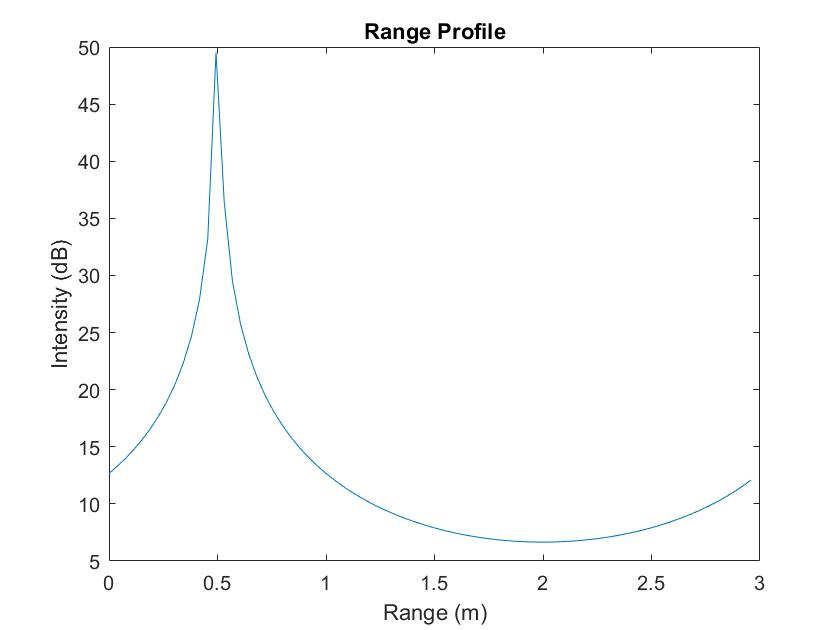
\includegraphics[width=0.7\linewidth]{chapters/chapter02/figures/range_profile}
	\caption{}
	\label{fig:range profile}
\end{figure}

\begin{subappendices}
	\section{Chapter 2 MATLAB Code}
	\lstinputlisting{chapters/chapter02/matlab_code/chapter02.m}
\end{subappendices}














